\documentclass[paper=a4,notitlepage,parskip=half,plainheadsepline]{scrartcl}

\usepackage{silence}
\WarningsOff[everypage]% Suppress warnings related to package everypage
\usepackage{snapshot} 
\usepackage{scrlayer-scrpage} 
\usepackage{iftex}
\usepackage[ngerman]{babel}
\usepackage{graphicx}
\usepackage{float}
\usepackage[T1]{fontenc}
\usepackage[utf8]{inputenc}
\usepackage{pifont}
\usepackage{amsmath}
\usepackage{textcomp}
\usepackage[german]{varioref}
\usepackage[text={6.8in,9.6in},top=0.7in,centering]{geometry}
\usepackage{datetime2}
\usepackage{array,multirow,tabularx}
\usepackage{listingsutf8}
\usepackage[table,svgnames,dvipsnames]{xcolor}
\usepackage[most,breakable,skins,listingsutf8]{tcolorbox}
%\tcbuselibrary{listingsutf8}
\usepackage[color=blue!90,scale=0.8,placement=bottom,vshift=1.2cm]{background}
\usepackage{array}
\usepackage{physics}
\usepackage{tikz}
\usepackage{pgfplots}
\usepgflibrary{shapes.symbols}
\usetikzlibrary{arrows}
\pgfplotsset{compat=1.16}

%%%%%%%%%%%%%%%%%%%%%%%%%%%%%%%%%%%%%%%%%%          Aufgabe oder Loesung 
\newif\ifloesung
%\loesungtrue
\loesungfalse
%%%%%%%%%%%%%%%%%%%%%%%%%%%%%%%%%%%%%%%%%%%%%%%%%%%%%%%%%%%%%%%%%%%%%%%%%

%\backgroundsetup{contents={Version vom \today}}
\backgroundsetup{contents={Version vom \today}}
%\pagestyle{empty}

\pagestyle{scrheadings}
\clearpairofpagestyles
\ihead{Fachinformatiker Anwendungsentwickler~/~Informatik--Studenten}
\chead{}
\ohead{C/Python Simulation}
\ifoot{Frank Zimmermann}
\cfoot{SVLFG}
\ofoot{}
\ofoot{\pagemark}

\graphicspath{{./jpg/}}
\DeclareGraphicsExtensions{.jpg,.eps,.png}
%\usepackage{courier}


%\newcommand\bashprompt{\textcolor{cyan}{\small\ttfamily\bfseries{bob@remotehost{\textcolor{black}:}\textcolor{cyan!60}{\url{~}}{\textcolor{black}\$ }}}}
\newcommand\bashprompt{\textcolor{red!25!white}{\small\ttfamily\bfseries bash\$> }}
\newcommand\noprompt{\hspace{0.6cm}}
\newcommand{\startBash}{\gdef\myprompt{\bashprompt}}
\newcommand{\startNone}{\gdef\myprompt{\noprompt}}

\newcommand{\mingw}{\textsl{MinGW}}
\newcommand{\bash}{\emph{bash}}
\newcommand{\msys}{\textsl{MSYS}}
\newcommand{\git}{\emph{Git}}
\newcommand{\gcc}{\emph{gcc}}
\newcommand{\listingsfont}{\ttfamily}

\RedeclareSectionCommand[
  beforeskip=-1\baselineskip,
  afterskip=.5\baselineskip]{section}
\RedeclareSectionCommand[
  beforeskip=-.75\baselineskip,
  afterskip=.5\baselineskip]{subsection}
\RedeclareSectionCommand[
  beforeskip=-.5\baselineskip,
  afterskip=.25\baselineskip]{subsubsection}
\RedeclareSectionCommand[
  beforeskip=.5\baselineskip,
  afterskip=-1em]{paragraph}
\RedeclareSectionCommand[
  beforeskip=-.5\baselineskip,
  afterskip=-1em]{subparagraph}

% Wenn pdflatex benutzt wird sollen die 
% installierten! frutiger-Fonts verwendet werden
% Ansonsten die TeX-eigenen cmbright
\ifPDFTeX %
\usepackage[scaled=0.90]{frutiger}
\renewcommand\familydefault{\sfdefault}
%\DeclareFixedFont\ott{T1}{phv}{mc}{n}{10pt
\else
\usepackage{cmbright}
\fi

\newfont{\lf}{svlfg scaled 2000}%
\newcolumntype{P}[1]{>{\centering\arraybackslash}p{#1}}

\ifloesung
\newtcbinputlisting[auto counter,list inside=lol,list type={lstlisting}]{\mylisting}[4][]{%
  toptitle=2mm,
  bottomtitle=2mm,listing only,
  colback=lightgray,
  %colback=yellow!10,
  listing file={#3},
  listing options={language=#4,
  aboveskip=5pt,
  belowskip=5pt,
  columns=flexible,
  keywordstyle=\color{blue},
  basicstyle=\footnotesize\listingsfont},
  colback=white,
  %colframe=gray!75!black,
  colframe=yellow!50!black,
  listing only,
  fonttitle=\bfseries,
  breakable,
  %title={Soubor \thetcbcounter: #2},
  title=Musterlösung für \texttt{#3},
  #1
}
\fi

\begin{document}
\tcbset{enhanced,colback=green!5!white, boxrule=0.5pt, colframe=green!35!black,fonttitle=\bfseries\Large}
        % \begin{tcolorbox}[drop lifted shadow]
        % This is a tcolorbox.
        % \end{tcolorbox}\par\bigskip
        \begin{tcolorbox}[toptitle=3mm,bottomtitle=3mm,title=\centering{{\lf J}\hfil FI Anwendungsentwicklung / Duales Studium\hfil {\lf J}},
          drop lifted shadow=gray]
        \centering{\vspace{0.5cm}\LARGE Programmierübung %
        \ifloesung (mit Musterlösung)\fi}\\[0.3cm]
        \centering{C/Python--Programmierung / Simulation / Nash--Gleichgewichte}\\\vspace{0.5cm}
        \end{tcolorbox}

\section{Szenario II}
In diesem Szenario gibt es 2 Firmen, die ein identisches Produkt auf den Markt bringen wollen.
Die Kosten für jede Firma zur Herstellung eines Produktes sind für jede Firma identisch ($c=3/2$).

Die Preise, zu denen die Firmen ihre Produkte auf den Markt bringen möchten ($p_1$ und $p_2$), stehen noch nicht fest.
Sie sollen aber so gestaltet werden, dass jede Firma einen optimalen Preis für sich selbst erzielen kann, der ihren Gewinn unter diesen Bedingungen maximiert, und eine stabile Marktsituation entstehen kann (\emph{Nash--Gleichgewicht}).

Eine Marktanalyse hat die Nachfrage nach diesem Produkt ermittelt $$D_i(p_i,p_j)=5 - 2 p_i + p_j \qquad i={1,2}, \qquad i\neq j$$.

D.h. für jede Firma gibt es die gleiche Nachfragefunktion und daher wird erwartet, dass beide Firmen zu einem gleichen Preis kommen, der aber für jede Firma optimal ist.

Auch hier können nur einmal zur Markteinführung die Preise $p_1$ und $p_2$ (simultan) festgelegt werden und bleiben dann unverändert.

\section{Aufgabe}
Ihre Aufgabe ist es, für ihr Unternehmen~1 einen optimalen Preis so zu kalkulieren, dass das Unternehmen~2 ebenfalls optimale Gewinne machen kann und beide Unternehmen dauerhaft auf dem Markt existieren können. 

Dabei bestimmt die jeweilige \emph{Nachfragefunktion}, wie häufig ihr Produkt bei Ihrer Firma erworben wird, abhängig von ihrem Preis $p_1$ und dem Preis Ihres Konkurrenten $p_2$.

Folgende Grafik (Abb.~\ref{fig:Gewinnfunktion} auf Seite~\pageref{fig:Gewinnfunktion}) zeigt die Gewinnfunktion ($G_1(p_1,p_2)$) für das Unternehmen~1, in der die Nachfragefunktion \linebreak[3] ($D_1(p_1,p_2)$) und die Kosten ($c=3/2$) einberechnet sind:

\begin{equation}
G_1(p_1,p_2) = D_1(p_1,p_2) (p_1 - 3/2) = (5 - 2 p_1 + p_2) (p_1-3/2) 
\end{equation}

\begin{figure}
\begin{center}
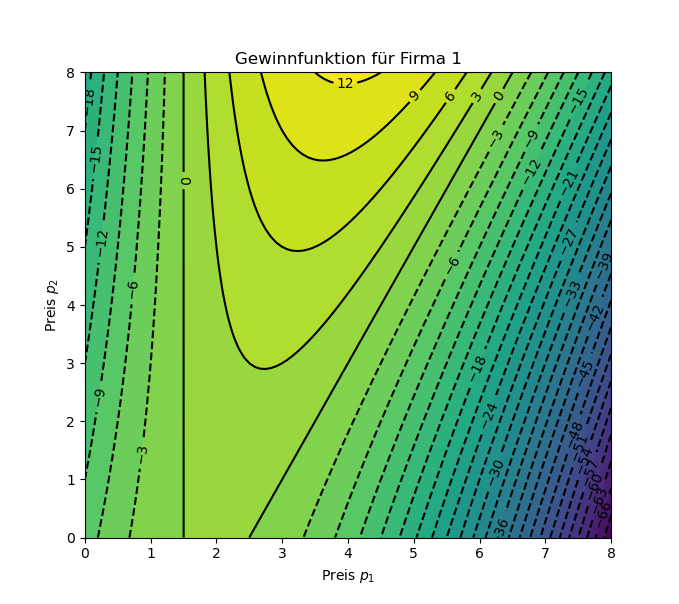
\includegraphics[width=0.7\textwidth]{nash2.png}
\end{center}
\caption{Gewinnfunktion aus Sicht des Unternehmens~1}
\label{fig:Gewinnfunktion}
\end{figure}

\begin{itemize}
\item Ermitteln Sie den maximalen Gewinn, den beide Unternehmen jeweils erzielen können.
\item Ermitteln Sie die Anzahl der vorgenommenen Käufe gemäß Marktanalyse zu diesen Preisen.
\item Ermitteln Sie den dazu notwendigen optimalen Preis.
\item Zeichnen Sie den Punkt in die Grafik ein.
\end{itemize}


\section{Hintergrund}
Die Aufgabe beschreibt ein sogenanntes \emph{Nash--Gleichgewicht}, bei dem beide Parteien eine optimale Strategie anwenden, wenn der Gegner ebenfalls bei seiner Strategie bleibt (\emph{kontinuierliche Strategien}). Das \emph{Nash--Gleichgewicht} gehört zum Bereich der \emph{Spieltheorie}.
Die Aufgabe ist ähnlich wie bei den diskreten \emph{Nash--Gleichgewichten} mit der Bimatrix, nur dass jetzt kontinuierliche Größen verwendet werden.

Dies ist ein klassischer Aufgabentyp in der VWL.

Entdecker dieses besonderen Gleichgewichts ist John Nash\footnote{John Forbes Nash, Jr., \textborn 13. Juni 1928 in Bluefield, West Virginia; \textdied 23. Mai 2015 nahe Monroe Township, New Jersey}, Hauptfigur des Filmes \emph{A Beautiful Mind}. In der Volkswirtschaftslehre gehört diese Aufgabenstellung in den Bereich der Mikroökonomie/Spieltheorie.

\section{Abgabe und Zeitrahmen}
Die Aufgabe ist \emph{optional} und kann jederzeit zwischendurch bearbeitet werden.
Interessant ist, wie genau die geforderten Werte (im Vergleich zur rechnerischen Lösung) bestimmt werden können.


\ifloesung
\newpage
\section{Musterlösung}
Beide Szenarien sind typische Aufgaben aus der Volkswirtschaftlehre im Bereich der Mikroökonomie.

Daher lassen sich beide Aufgaben sowohl analytisch lösen als auch per Simulation.

Eine Musterlösung in \emph{Python} zu beiden Szeanarien findet sich zum Ende dieses Papiers.

\section{Die analytische Lösung}
\subsection{Unterschied zwischen den Szenarien}
Beide Aufgaben scheinen auf den ersten Blick recht ähnlich zu sein, aber der Unterschied zwischen den Szenarien ist wichtig.

In beiden Szenarien ist die Grundlage immer die Gewinnfunktion\footnote{auch \emph{Zielfunktion}, \emph{Auszahlungsfunktion} 
oder \emph{Nutzenfunktion} genannt}, die in diesem Problem von den Preisen, der Nachfragefunktion und den Kosten abhängt ($G(D_i,p_i,c_i)$). 

$$D_i(p_i, p_j) \qquad i={1,2} \quad i\neq j \qquad \text{Nachfragefunktion (Demand function)} $$

Diese Nachfragefunktion kann von \emph{keinem} der beiden Preise, von \emph{einem} oder von \emph{beiden} Preisen abhängig sein.

Im ersten Szenario ist die Nachfragefunktion für beide Unternehmen nur von dem eigenen Preis abhängig.
Bei gleichen Kosten ($c_1=c_2=c=3/2$) muss aus Symmetriegründen dann der Preis für beide Unternehmen derselbe sein ($p_1=p_2=p$).
Daher muss der gesuchte Preis genau auf der Winkelhalbierenden zwischen der $p_1$--Achse und der $p_2$--Achse liegen.

Im zweiten Szenario hat jedes Unternehmen ebenfalls die gleiche Nachfragefunktion (daher muss auch hier der gesuchte Extremwert auf der Winkelhalbierenden liegen), aber die Nachfragefunktion hängt diesmal von beiden Preisen ab.

Das gesuchte Extremum ist daher nicht einfach ein Punkt auf der $p_1$--Achse, der eine vertikale Linie definiert (wie in Szeanrio~I), 
sondern für jeden Preis $p_2$ gibt es einen anderen Extrempunkt für $p_1$. Der Preis $p_2$ ist hier ein Parameter, der die Lage des Extremwertes beeinflusst.
Die Linie der Extrempunkte ist hier eine geneigte Gerade.

In beiden Fällen findet man wegen der Symmetrie den gewünschten Punkt maximalen Gewinns in der 2--dimensionalen Gewinnfunktion als 
Schnittpunkt zwischen der Linie der Extrempunkte einerseits und der Winkelhalbierenden zwischen $p_1$--Achse und $p_2$--Achse andererseits.

 In der Grafik der Gewinnfunktionen weiter unten (Abb.~\ref{fig:Doppelgrafik}~auf Seite~\pageref{fig:Doppelgrafik}) ist daher in jeder Grafik die Linie der Extrempunkte als auch die Winkelhalbierende eingezeichnet.

 Der Schnittpunkt dieser beiden Linien definiert dann den Punkt maximalen Gewinns im Nash--Gleichgewicht.

\subsection{Szenario I}
Hier lautet die Nachfragefunktion für Unternehmen~1

$$D_1(p_1,p_2)= 5-p_1 = 5-p_2 = 5-p$$

Damit erhalten wir als Gewinnfunktion, wenn wir die Nachfrage mit dem Nettogewinn des Produktes \linebreak[5] $(p_1-c_1)=(p-c)$ multiplizieren

$$G(p_1,p_2) = (5-p) (p-c) = 5p -5c -p^2 +pc = -p^2 + (5+c)p -5c$$

Dies ist eine umgekehrte Parabel, die genau ein Maximum für $p$ besitzt. Setzt man für $c=3/2$ ein, so erhält man
den Extremppunkt $p_E$ (nach Ableitung und Nullsetzung)
$$ p^*_E = \frac{13}{4}$$

Dieser ist völlig unabhängig vom Preis $p_2$ und stellt den Preis dar, bei dem die Gewinnfunktion maximal wird.
Die Linie des Extrempunktes in der Gewinnfunktion ist hier, wegen der Unabhängigkeit von $p_2$,  einfach eine vertikale Linie, weil sie für jeden möglichen
 Preis von $p_2$ gilt.

Aus Symmetriegründen gilt dieser Preis dann auch für das Unternehmen~2 und daher liegt der endgültige Preis beider Unternehmen auch auf der Winkelhalbierenden.

\subsection{Szenario II}
Hier ist die Nachfragefunktion von beiden Preisen abhängig:

$$D_1(p_1,p_2) = 5 - 2 p_1 + p_2$$

Beim zweiten Szenario ist der maximale Gewinn für das Unternehmen~1 sowohl vom Preis $p_1$ des Unternehmens~1 
als auch vom Preis $p_2$ des Unternehmens~2 abhängig. Dies macht die Lage deutlich komplizierter. 
Nun müssen wir einen Gleichgewichtspreis suchen, der für beide Unternehmen optimal ist.

Um hier den Extrempunkt der Gewinnfunktion $G_1(p_1,p_2)$ zu finden müssen wir partiell nach der Variablen $p_1$ ableiten und dabei $p_2$ einfach als einen
konstanten Parameter betrachten. Der Extrempunkt ist dann wie gewohnt durch Nullsetzen dieser Ableitung zu finden.

$$G_1(p_1,p_2)= (5- 2 p_1 + p_2) (p1-3/2)  = -2 p_1^2 + (5+3+p_2) p_1 - \frac{15}{2} - \frac{3}{2}p_2$$

Leitet man partiell ab

$$\frac{\partial G_1(p_1,p_2)}{\partial p_1} = -4 p_1 + (5+3+p_2)$$

und setzt gleich Null erhält man die Extremwerte mit $p_2$ als weiteren Parameter:

$$ -4 p_1 + (8+p_2) = 0     \qquad \Rightarrow \qquad p_{1E} = \frac{8+p_2}{4}$$

Schreibt man das um und betrachtet $p_2$ als y--Variable erkennt man übrigens die Geradengleichung, auf der sich die Extrempunkte befinden.

$$p_2 = 4 \ p_{1E} -8$$

Eine Gerade mit $4$--facher Steigung und $-8$ Achsenabschnitt ist in der rechten Grafik (Abb.~\ref{fig:Doppelgrafik}~auf Seite~\pageref{fig:Doppelgrafik}) eingezeichnet.

Der Schnittpunkt mit der Winkelhalbierenden zwischen $p_1$--Achse und $p_2$--Achse ist dann der gesuchte Punkt für den maximalen Gewinn im \emph{Nash--Gleichgewicht}. 
Rechnerisch findet man ihn durch Gleichsetzen von $p_{1E}$ und $p_2$:\footnote{Extremwerte, die Werte im Nash--Gleichgewicht repräsentieren werden üblicherweise mit einem Sternchen ($^*$) gekennzeichnet}

$$p^*_{1E} = \frac{8}{3}$$

\subsection{Weitergehendes}
Für den Interessierten an solchen Fragestellungen und Lösungen aus der Spieltheorie:

Dieses Szenario findet man unter dem Begriff \emph{Cournot\footnote{Antoine-Augustin Cournot \textborn 28. August 1801 in Gray; \textdied 31. März 1877 in Paris}--Nash} bzw. \emph{Oligopol/Duopol} in der Fachliteratur.

Prinzipiell geht man oft wie folgt vor (Rezept für Duopol):

\begin{enumerate}
\item Aufstellen der Nachfrage--Funktion
\item Aufstellen der Kostenfunktion
\item Konstruieren der Zielfunktion/Gewinnfunktion!
\item Durch partielles Ableiten ein parametrisiertes Extremum finden ($f(p_2)$)
\item Bei symmetrischen Problemen ist man damit am Ende:
\subitem Da die \emph{beste Antwort}/\emph{Reaktionsfunktion}  $p^*_1\stackrel{Nash}{=}R_1(p^*_2)= f(p^*_2)$ \ldots
\subitem \ldots kann man $p^*_1=p^*_2=p^*$ setzen und auflösen.
\item Bei Nicht--Symmetrischen Problemen:
\subitem Reaktionsfunktion (\emph{Beste Antwort}) aus der Ableitung konstruieren $R_1(p_2)= f(p_2)$
\item Für Nash--Gleichgewicht gilt dann wegen $R_1(p^*_2) = p^*_1 \quad\text{und}\quad R_2(p^*_1) = p^*_2$:
\subitem $p^*_1 \stackrel{Nash}{=} R_1(p^*_2) \stackrel{Nash}{=} R_1(R_2(p^*_1))$
\subitem Auflösen nach $p^*_1$ und einsetzen, um $p^*_2$ zu bekommen. 
\end{enumerate}

\newpage
\section{Das Programm für Szenario I und II}
\lstset{ % General setup for the package
%     language={C},
%     basicstyle=\small\sffamily,
     numbers=left,
     numberstyle=\tiny,
%     frame=tb,
%     tabsize=4,
%     columns=fixed,
     showstringspaces=true,
     numbersep=5pt,
%     showtabs=false,
%     keepspaces,
     commentstyle=\color{olive},
     inputencoding=utf8/latin1
%     keywordstyle=\color{blue}
}%
\begin{figure}
\begin{center}
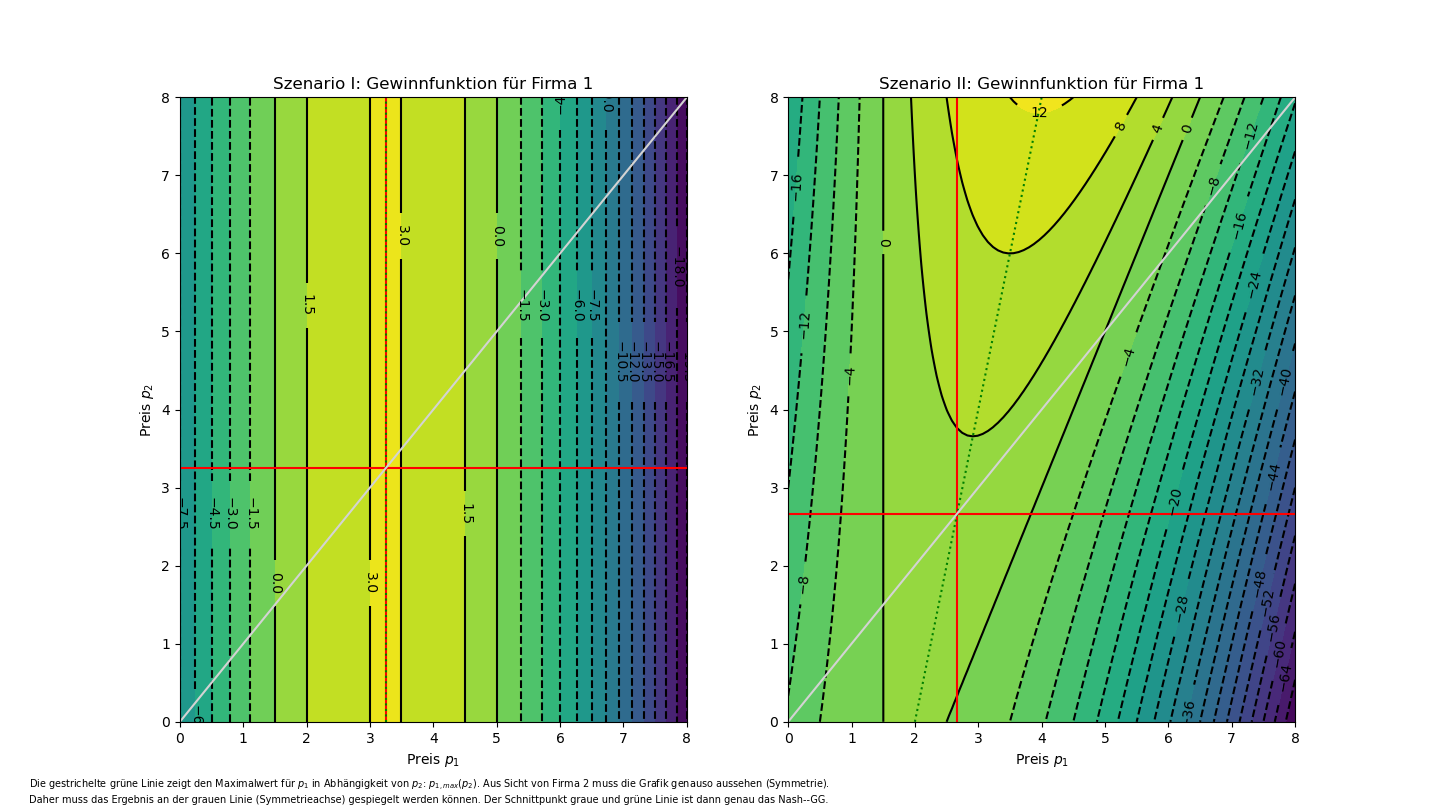
\includegraphics[width=1.02\textwidth]{nashBoth.png}
\caption{Gewinnfunktionen für Szenario I (links) und Szenario II (rechts)}
\label{fig:Doppelgrafik}
\end{center}
\end{figure}

\mylisting[label=musterloesung1]{Musterlösung}{nash.py}{python}
\fi
\end{document}